\documentclass[12pt,a4paper]{article}
\usepackage[utf8]{inputenc}
\usepackage[french]{babel}
\usepackage[T1]{fontenc}
\usepackage{amsmath}
\usepackage{amsfonts}
\usepackage{amssymb}
\usepackage{graphicx} 
\usepackage[left=2cm,right=2cm,top=2cm,bottom=2cm]{geometry}

\author{Pierre BIDAULT \& Matthias GOFFETTE}
\title{Modélisation pour Feudal Overlords}

\begin{document}
\maketitle

\section{Cas d'utilisation}

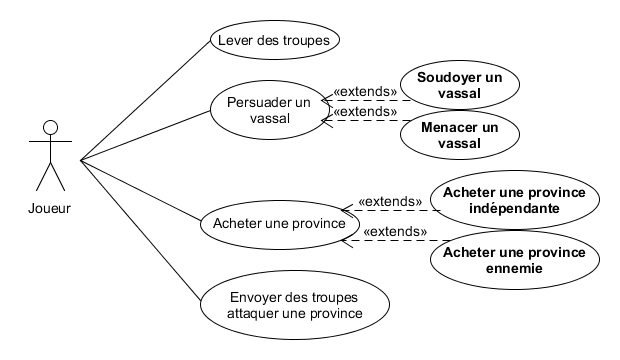
\includegraphics[scale=0.7]{Diagramme_Cas_Utilisation/Diagramme_Cas_Utilisation.png}

\newpage

\section{Pré- et Post-conditions des Cas d'utilisation}

\begin{itemize}
\item Cas numéro 1 : Lever des Troupes
	\begin{itemize}
	\item Précondition : Troupes disponibles > 0 $ \land $ Territoire appartient au joueur courant
	\item Postcondition : Le joueur courant a ajouté Troupes disponibles à son total
	\end{itemize}
\item Cas numéro 2 : Persuader un vassal
	\begin{itemize}
	\item Précondition : La méthode choisie est valide $ \land $ le vassal s'est rebellé $ \land $ le joueur dispose de suffisamment de ressources
	\item Postcondition : Le vassal n'est plus rebelle $ \land $ le joueur a dépensé les ressources nécessaires
	\end{itemize}
\item Cas numéro 3 : Acheter une province
	\begin{itemize}
	\item Précondition : Le joueur a assez d'argent $ \land $ le vassal apprécie suffisamment le joueur $ \lor $ le joueur détenant la province accepte
	\item Postcondition : Le vassal appartient désormais au joueur ayant acheté la province $ \land $ ce dernier a perdu la quantité d'argent correspondant au prix
	\end{itemize}
\end{itemize}

\newpage

\section{Préparation des tests unitaires}

\begin{table}[htbp!]
\begin{tabular}{|p{0.6\linewidth}|c|c|c|c|}
\hline 
Numéro de test
&1&2&3\\ 
\hline 
\hline
Précondition 1
&F&T&T\\ 
\hline
Précondition 2
& &F&T\\
\hline
\hline
Troupes levées
&F&F&T\\
\hline
\hline
Nombre de jeux de test
&X&X&X\\
\hline 
\end{tabular} 
\caption{Cas d'utilisation <<~Lever des troupes~>>}
\end{table}

\newpage

\section{Diagramme de Classes}

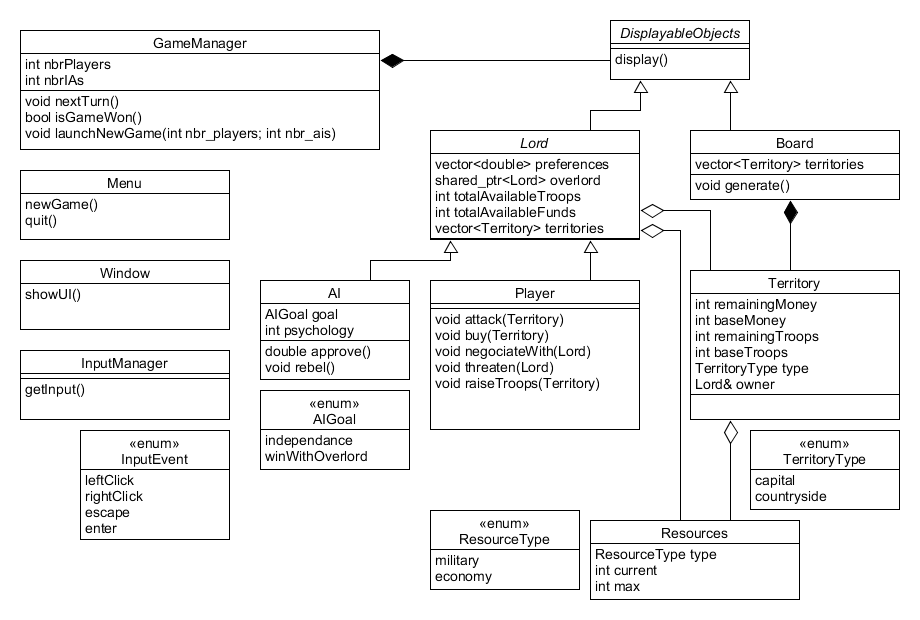
\includegraphics[scale=0.5]{Diagramme_Classes/diagramme_classes.png} 

\end{document}